\section{Data Modeling in Dataspace Support Systems}

In the paper ``Data Modeling in Dataspace Support Systems'' \cite{DBLP:conf/birthday/SarmaDH09}, the authors face the issue of uncertainty in dataspaces. In their view, a dataspace needs to model uncertainty in its core. In their work, they described the concepts of probabilistic mediated schemas and probabilistic mappings as enabling concepts for DSSPs. With this foundation, it is possible to completely bootstrap a pay-as-you-go integration system.

Current data integration systems are essentially a natural extension of traditional databases in that queries are specified in a structured form and data is modeled in one of the traditional data models like relational or XML. The System for data integration also has exact information about how the data in the sources map to the schema used for integration. So, for data integration there is a need for large upfront effort in creating the mediated schema and the schema mappings. Dataspace Support Platforms (DSSP) shall considerable reduce this upfront effort. The system should be able to bootstrap itself and provide useful services with no human intervention. When the data management needs become clearer (through user feedback or as sources are added), the system evolves in a pay-as-you-go fashion. 
In order to develop DSSPs, it is impossible to rely on the same data modeling paradigms data integration systems use. One cannot assume, that the mediated schema is given in advance and that the schema mappings between the sources and the mediated schema will be accurate. Therefore the authors argue that uncertainty has to be considered in the mediated schema and in the schema mappings.

\subsection{Uncertainty in Data integration}

\textbf{Sources of Uncertainty}

\uline{Uncertain mediated schema:} The set of schema terms in which queries are posed is called the mediated schema. Not necessarily they cover all the attributes in any source, it cover rather the aspects of the domain that the developer of the application wishes to expose to the user. For several reasons uncertainty happens in the mediated schema. First, if the mediated schema is derived from the data sources during bootstrapping, there will be some uncertainty about the results. When domains are broad, there will be also some uncertainty about how to model them, because in general, there will be overlappings in different topics. 

\uline{Uncertain schema mapping:} Schema mapping defines the semantic relationships between the terms in the sources and the terms used in the mediated schema. Although, schema mappings can be inaccurate. In a dataspace, many of the initial schema mappings are properly automatically derived, and therefore they may inaccurate. In general, it is impossible to create and maintain precise mappings between data sources. 

\uline{Uncertain data:} Some of the data may be obtained by automatisms as data sources may not always be structured well. Additionally, unreliable or inconsistent data may be contained in systems with many sources. 

\uline{Uncertain queries:} Properly, much of the early interaction with a dataspace will be done through keyword queries as the users aren't aware of a (non-existent) schema. The queries have to be translated into some structured form so they can be reformulated with respect to the data sources. At this point, multiple candidate structured queries could be generated and thus some uncertainty arises about which query captures the real intention of the user.

\subsection{System architecture}

The most fundamental characteristic of this system is that it is based on a probabilistic data model. In contrast to a traditional data integration system, which includes a single mediated schema and assumes a single (and correct) schema mapping between the mediated schema and each source, the data integration module of a DSSP attaches possibilities to multiple tuples, mediated schemas, schema mappings and possible interpretations of  keyword queries posed to the system. 

For DMS it is assumed that queries are posed as keywords. This is contrary to traditional integration systems which assume the query to be posed in a structured fashion( i.e. that it can be translated to some subset of SQL). So, a DSSP must first reformulate a keyword query into a set of candidate structured queries, before it can reformulate the query onto the schemas of the data sources. This step is also called keyword reformulation.  It is important to note, that keyword reformulation differs from keyword search techniques on structured data (see \cite{994693}, \cite{Hristidis:2002:DKS:1287369.1287427}) in that (a) it does not assume access to all data in the sources or that the sources support keyword search, and (b) it tries to distinguish different structural elements in the query in order to pose more precise queries to the sources. In any case, keyword reformulation should benefit from techniques that support answering search on structured data.

\begin{figure}[H]
	\begin{center}
		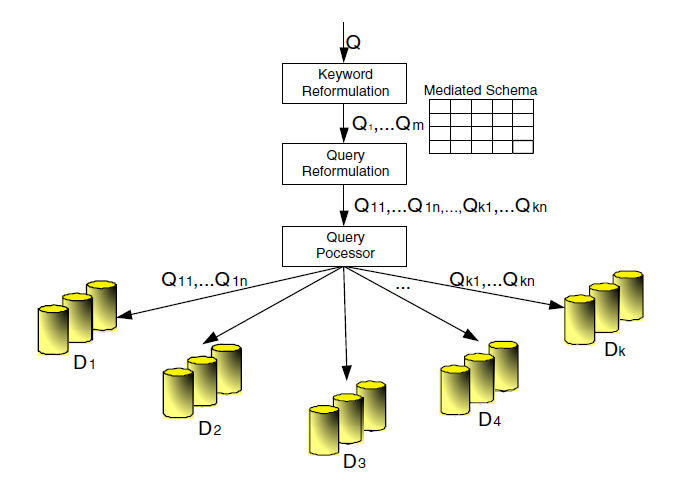
\includegraphics[width=0.75\textwidth]{figures/DataModelingInDSSPs-Figure1.png}
	\end{center}
	\caption{Architecture of a data integration system that handles uncertainty}
	\label{DataModelingInDSSPsFigure1}
\end{figure}

Different is also the query answering in a DSSP. It doesn't find necessarily all answers on a given query, rather than typically find the top-k answers, and rank these answers most effectively. 
The architecture of the proposed system is shown in \ref{DataModelingInDSSPsFigure1}. The DSSP contains a number of data sources and a mediated schema (probabilistic mediated schemas are omitted here). When the user poses a query, which can be either a structured or a keyword query, the systems returns a set of answer tuples, each with a calculated probability. If a keyword query was posed, a keyword reformulation has firstly be done to translate it into a set of candidate structured queries on the mediated schema. Otherwise, the candidate query is the posed query itself.